\documentclass{article}
\usepackage{graphicx} % Required for inserting images
\usepackage{amsmath}  % improve math presentation
\usepackage{gensymb} % added so I have the degree symbol
\usepackage[margin=1in,letterpaper]{geometry} % decreases margins
\usepackage[final]{hyperref} % adds hyper links inside the generated pdf file
\usepackage{physics} %use for mathematical symbols
\usepackage[backend=biber,style=alphabetic,sorting=ynt]{biblatex}
\addbibresource{refs_figures/refs.bib}
\title{Polarimeter Manual}
\author{Deven Bowman}
\date{May 2023}

\begin{document}

\maketitle

\begin{figure}[h]
    \centering
    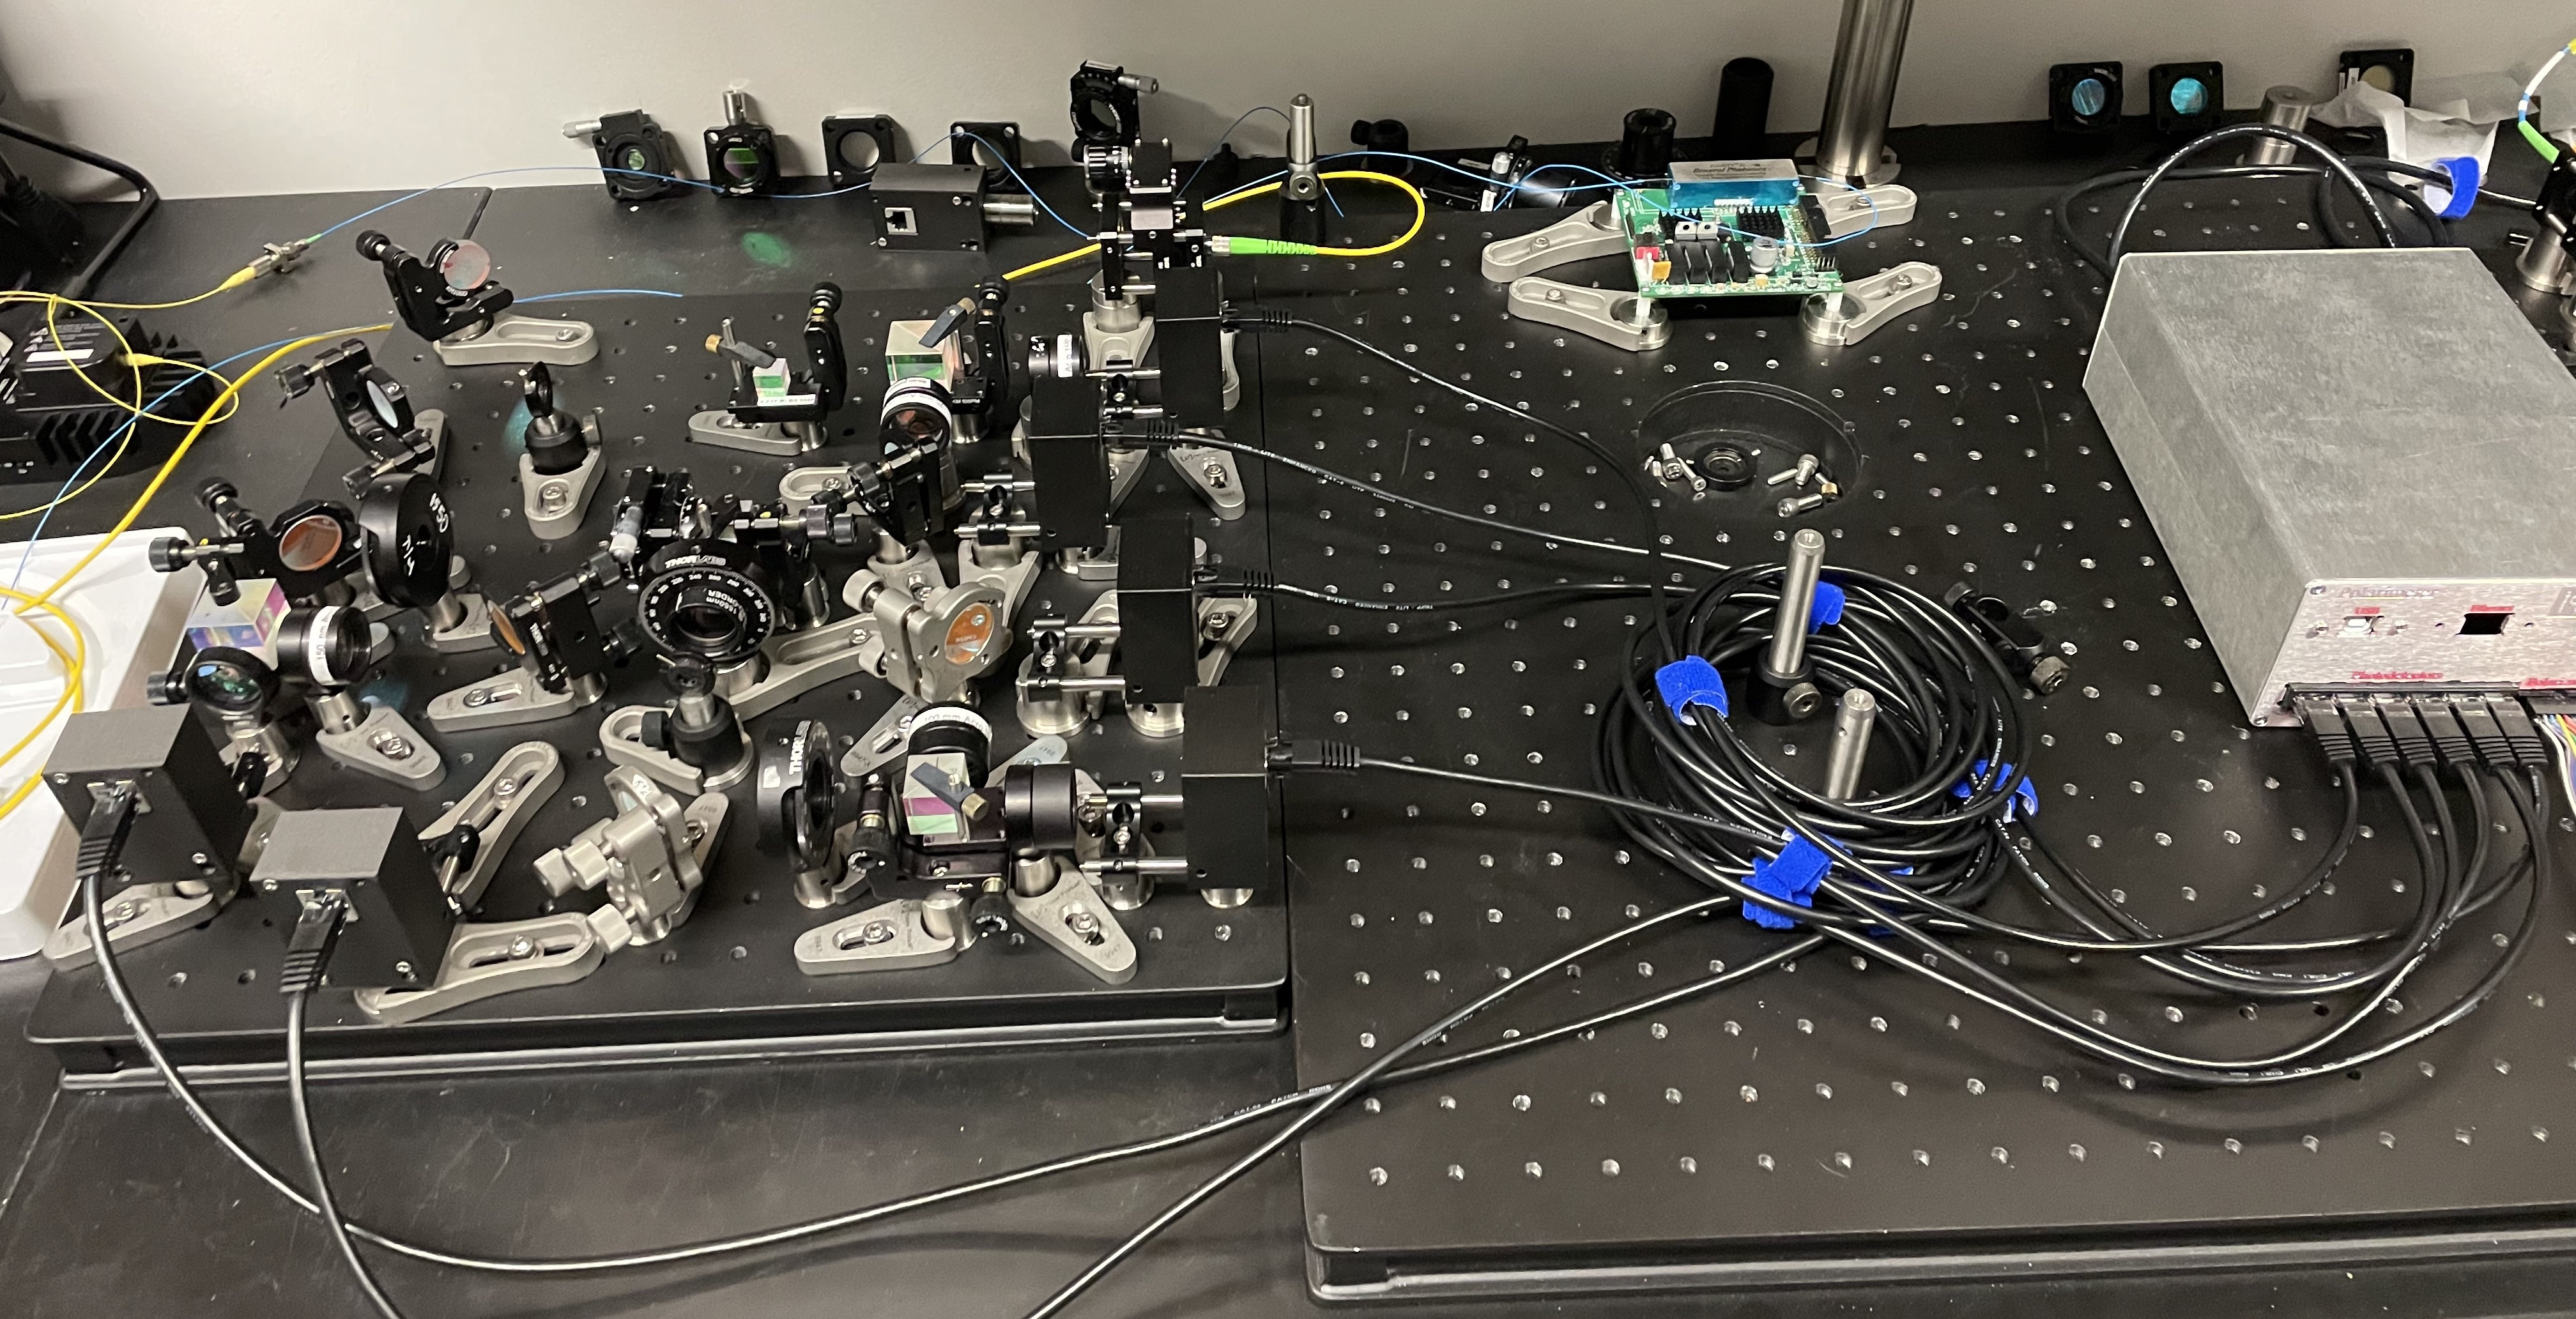
\includegraphics[width = \textwidth]{refs_figures/Polarimeter Overview.jpg}
    % \caption{1550 nm polarimeter}
    \label{Polarimeter_pic}
\end{figure}


\section{How it works}
\subsection{A review of Stokes Parameters}
The Stokes parameter description of polarization uses 4 intensity based metrics to fully describe any full or partially polarized state. Stokes parameters are based solely on observables which makes them the description to use when measuring a polarization state.

\begin{equation}
    \Vec{S}= \begin{bmatrix}
    S_0\\
    S_1\\
    S_2\\
    S_3\\
    \end{bmatrix}
    \label{Stokes Vector}
\end{equation}

These 4 parameters in Eq. \ref{Stokes Vector} are calculated with simple intensity measurements. $S_0$ is the total intensity of the light. $S_1$ measures the tendency of light to be horizontally polarized($H$), $S_1 > 0$, or vertically polarized($V$), $S_1 < 0$. $S_2$ measures the tendency of the light to be linearly polarized in the $45\degree$ or $-45\degree$ directions with $S_2 >0$ or $S_2<0$ respectively. $S_3$ describes the tendency of the light to be right circularly polarized($R$), $S_3 >0$, or left circularly polarized($L$), $S_3<0$. A Stokes vector can be written from these parameters to represent any pure or mixed polarization state. 
\subsection{Pure Polarization States}
\begin{figure}[!h]
\begin{center}
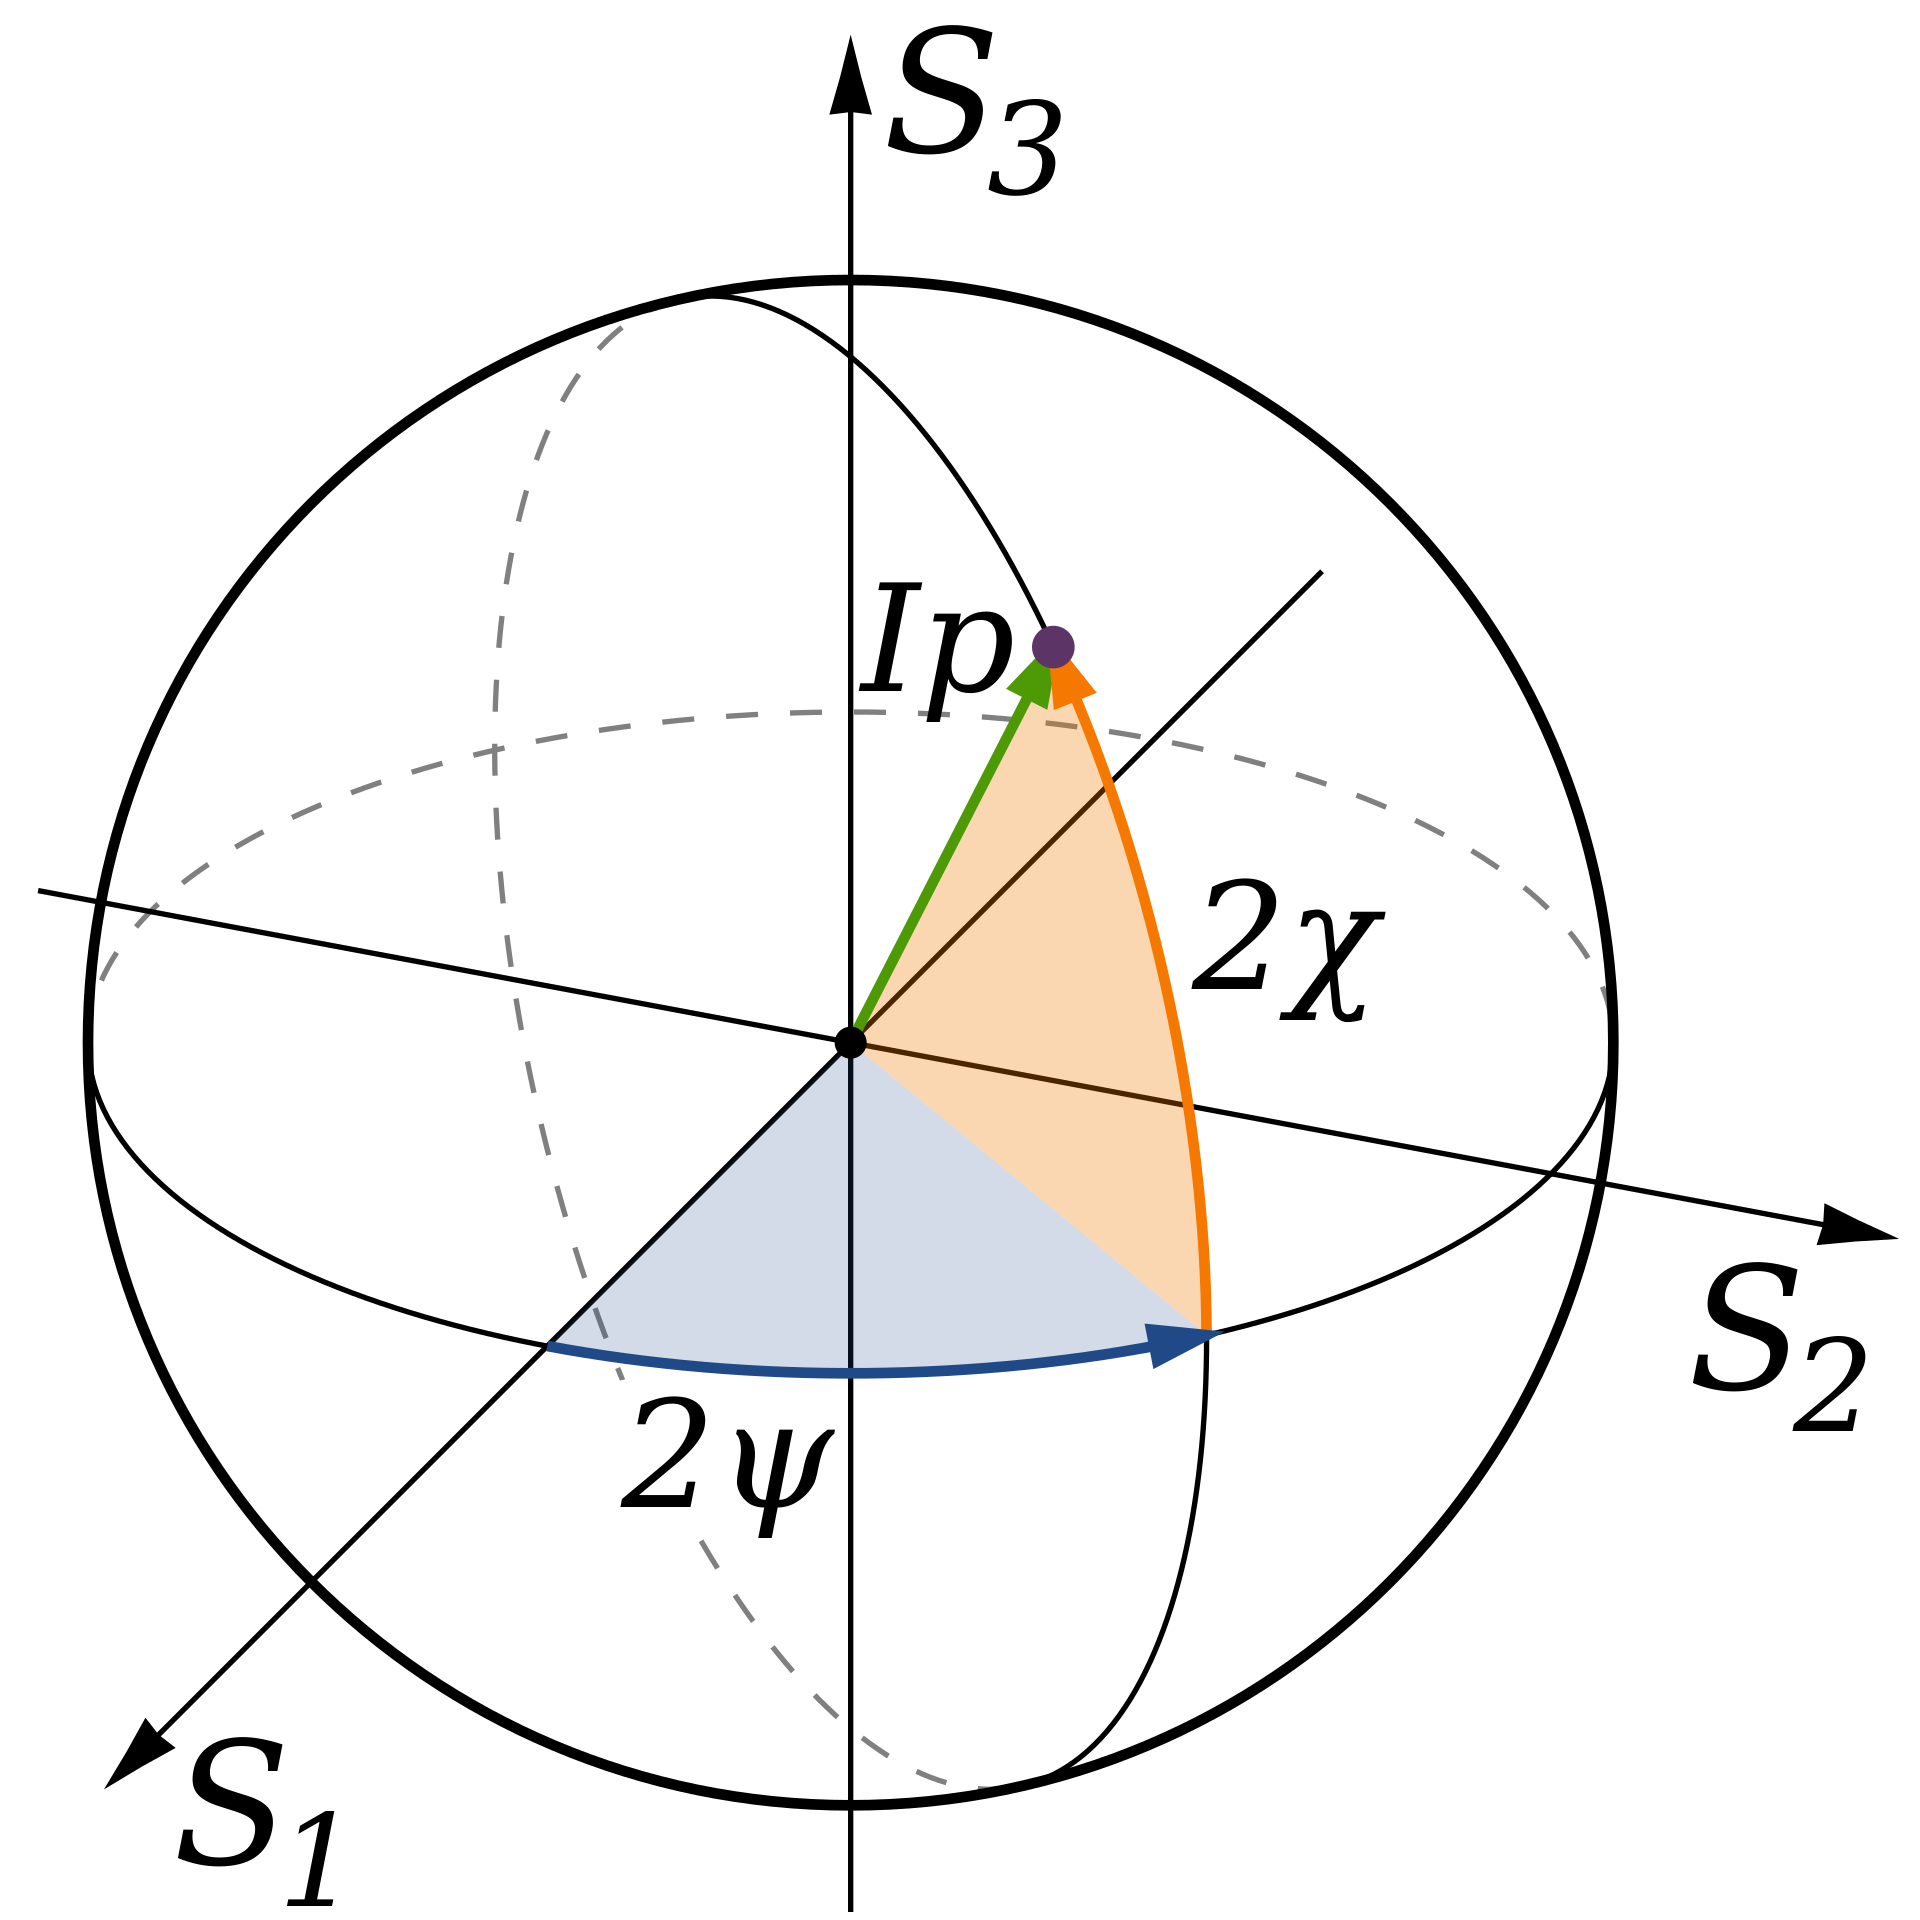
\includegraphics[width=0.4\textwidth]{refs_figures/Poincare_sphere.png}
\end{center}
\caption{The Poincare sphere and polarization ellipse angles $\psi$ and $\chi$ are displayed.}
\label{Poincare Sphere}
\end{figure}

For pure states, we have the property that $S_0^2=S_1^2+S_2^2+S_3^2$. As a result, Stokes vectors are often normalized by $S_0$ and reduced to a 3D unit vector.
\begin{equation}
    \Vec{S}= \frac{1}{S_0}\begin{bmatrix}
    S_1\\
    S_2\\
    S_3\\
    \end{bmatrix}
\end{equation}
It follows that the set of all pure polarization states can be mapped to a sphere. This mapping is known as the Poincare sphere and is displayed in Figure \ref{Poincare Sphere}. States on the Poincare sphere can be more concisely represented in terms of two angles.
\begin{equation}
    \psi = \frac{1}{2}\arctan{\frac{S_2}{S_1}}, \psi\in\{0^{\circ}, 180^{\circ}\}
\end{equation}
\begin{equation}
    \chi = \frac{1}{2}\arctan{\frac{S_3}{\sqrt{S_1^2 + S_2^2}}}, \chi\in\{-45^{\circ}, 45^{\circ}\}
\end{equation}
These angles are formulated to describe the polarization ellipse, but $2\psi$ and $2\chi$ are the spherical coordinate angles on the Poincare sphere. The factors of two represent that the same polarization state is represented when the polarization ellipse is rotated by $180^{\circ}$ and when the semi-major and semi-minor axes are swapped.


\subsection{Polarimeter Design}
The schematic diagram for the polarimeter is shown in figure \ref{Polarimeter Schematic}. This design uses six intensity measurements that are related to the Stokes parameters through a calibration matrix. The photodiode detectors are paired into three detection arms. Light incident on the polarimeter is split into these 3 detection arms by two non polarizing beam splitters, BS$_1$ and BS$_2$. Each detection arm has a series of waveplates, depicted as WP$_1$, WP$_2$ and WP$_3$, that apply transformations to the polarization state before reaching a polarizing beam splitter, PBS$_1$, PBS$_2$, and PBS$_3$, that transmits the projection of the state onto the vertical axis and reflects the projection onto horizontal axis. Finally, a pair of photodiode detectors measures the intensity at each output port of the polarizing beams splitters and produces a voltage signal. The polarization states which the beams splitters project onto is determined by the configuration of the preceding waveplates. The Stokes parameters describe the polarization state relative to 3 linearly independent axes. Therefore, waveplates are set to give us 3 linearly independent projection axes for the different detector arms. Furthermore, the farther spread out the projection axes are in Stokes space, the better the resolution the detector has achieve. 
\begin{figure}[!h]
\begin{center}
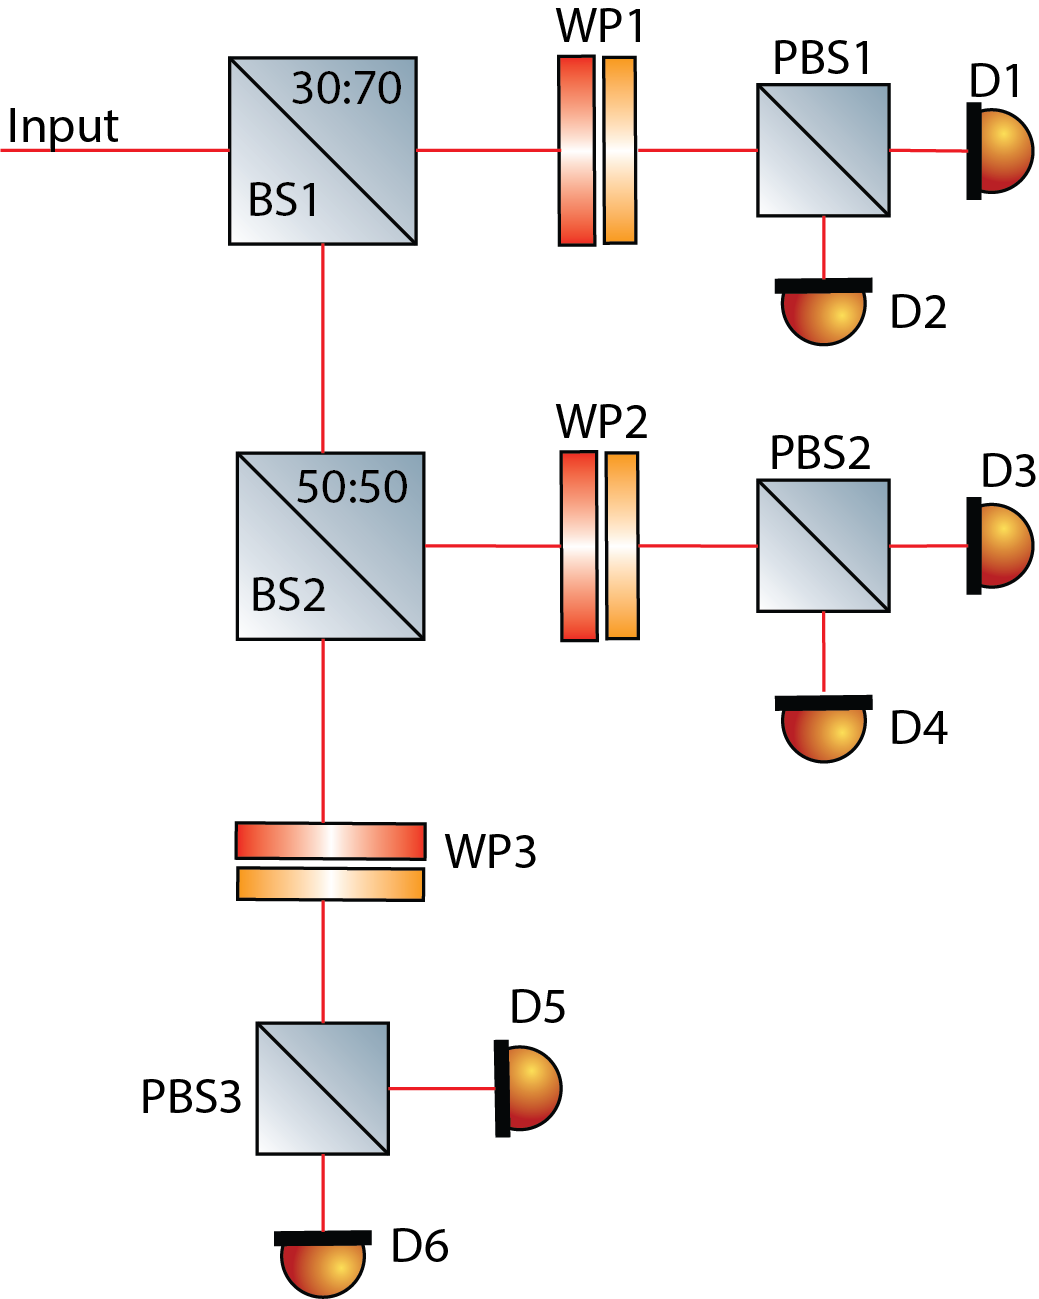
\includegraphics[width=0.5\textwidth]{refs_figures/PolarimeterSchematic.png}
\end{center}
\caption{The design for the Stokes Polarimeter uses several beam splitters (BS), waveplates (WP), polarizing beam splitters (PBS), and photodiode detectors (D) to measure the four Stokes parameters.}
\label{Polarimeter Schematic}
\end{figure}

To calculate the Stokes parameters from the output voltage signals, a matrix is calculated from a calibration procedure similar to that presented by Azzam and Lopez\cite{Azzam89}. 

\subsection{Calibration Matrix}
For a polarization state with Stokes vector $\vec{S}$, the polarimeter will generate 6 voltages we can write in a vector $\vec{V}$. The two are related by a 6 x 4 instrument matrix $\textbf{B}$ .
\begin{equation}
    \vec{V} = \textbf{B}\vec{S}
    \label{Calibration eq}
\end{equation} 
By generating well defined input polarization states, $\vec{S}$ and then measuring the resulting $\vec{V}$, the instrument matrix $\textbf{B}$ can be determined. Then, the Moore-Penrose left inverse of the instrument matrix, $\textbf{B}^{+}$ can be calculated.
\begin{equation}
    \textbf{B}^{+} = \textbf{B}^{T}(\textbf{B}\textbf{B}^{T})^{-1}
    \label{MP_inverse}
\end{equation}
Here, $\textbf{B}^{T}$ denotes the transpose of the matrix. This then allows the stokes vector of the incident light to be determined from the measured voltages: $\textbf{B}^{+}\vec{V}=\vec{S}$.


\section{How to Operate}
\begin{figure}[h]
    \centering
    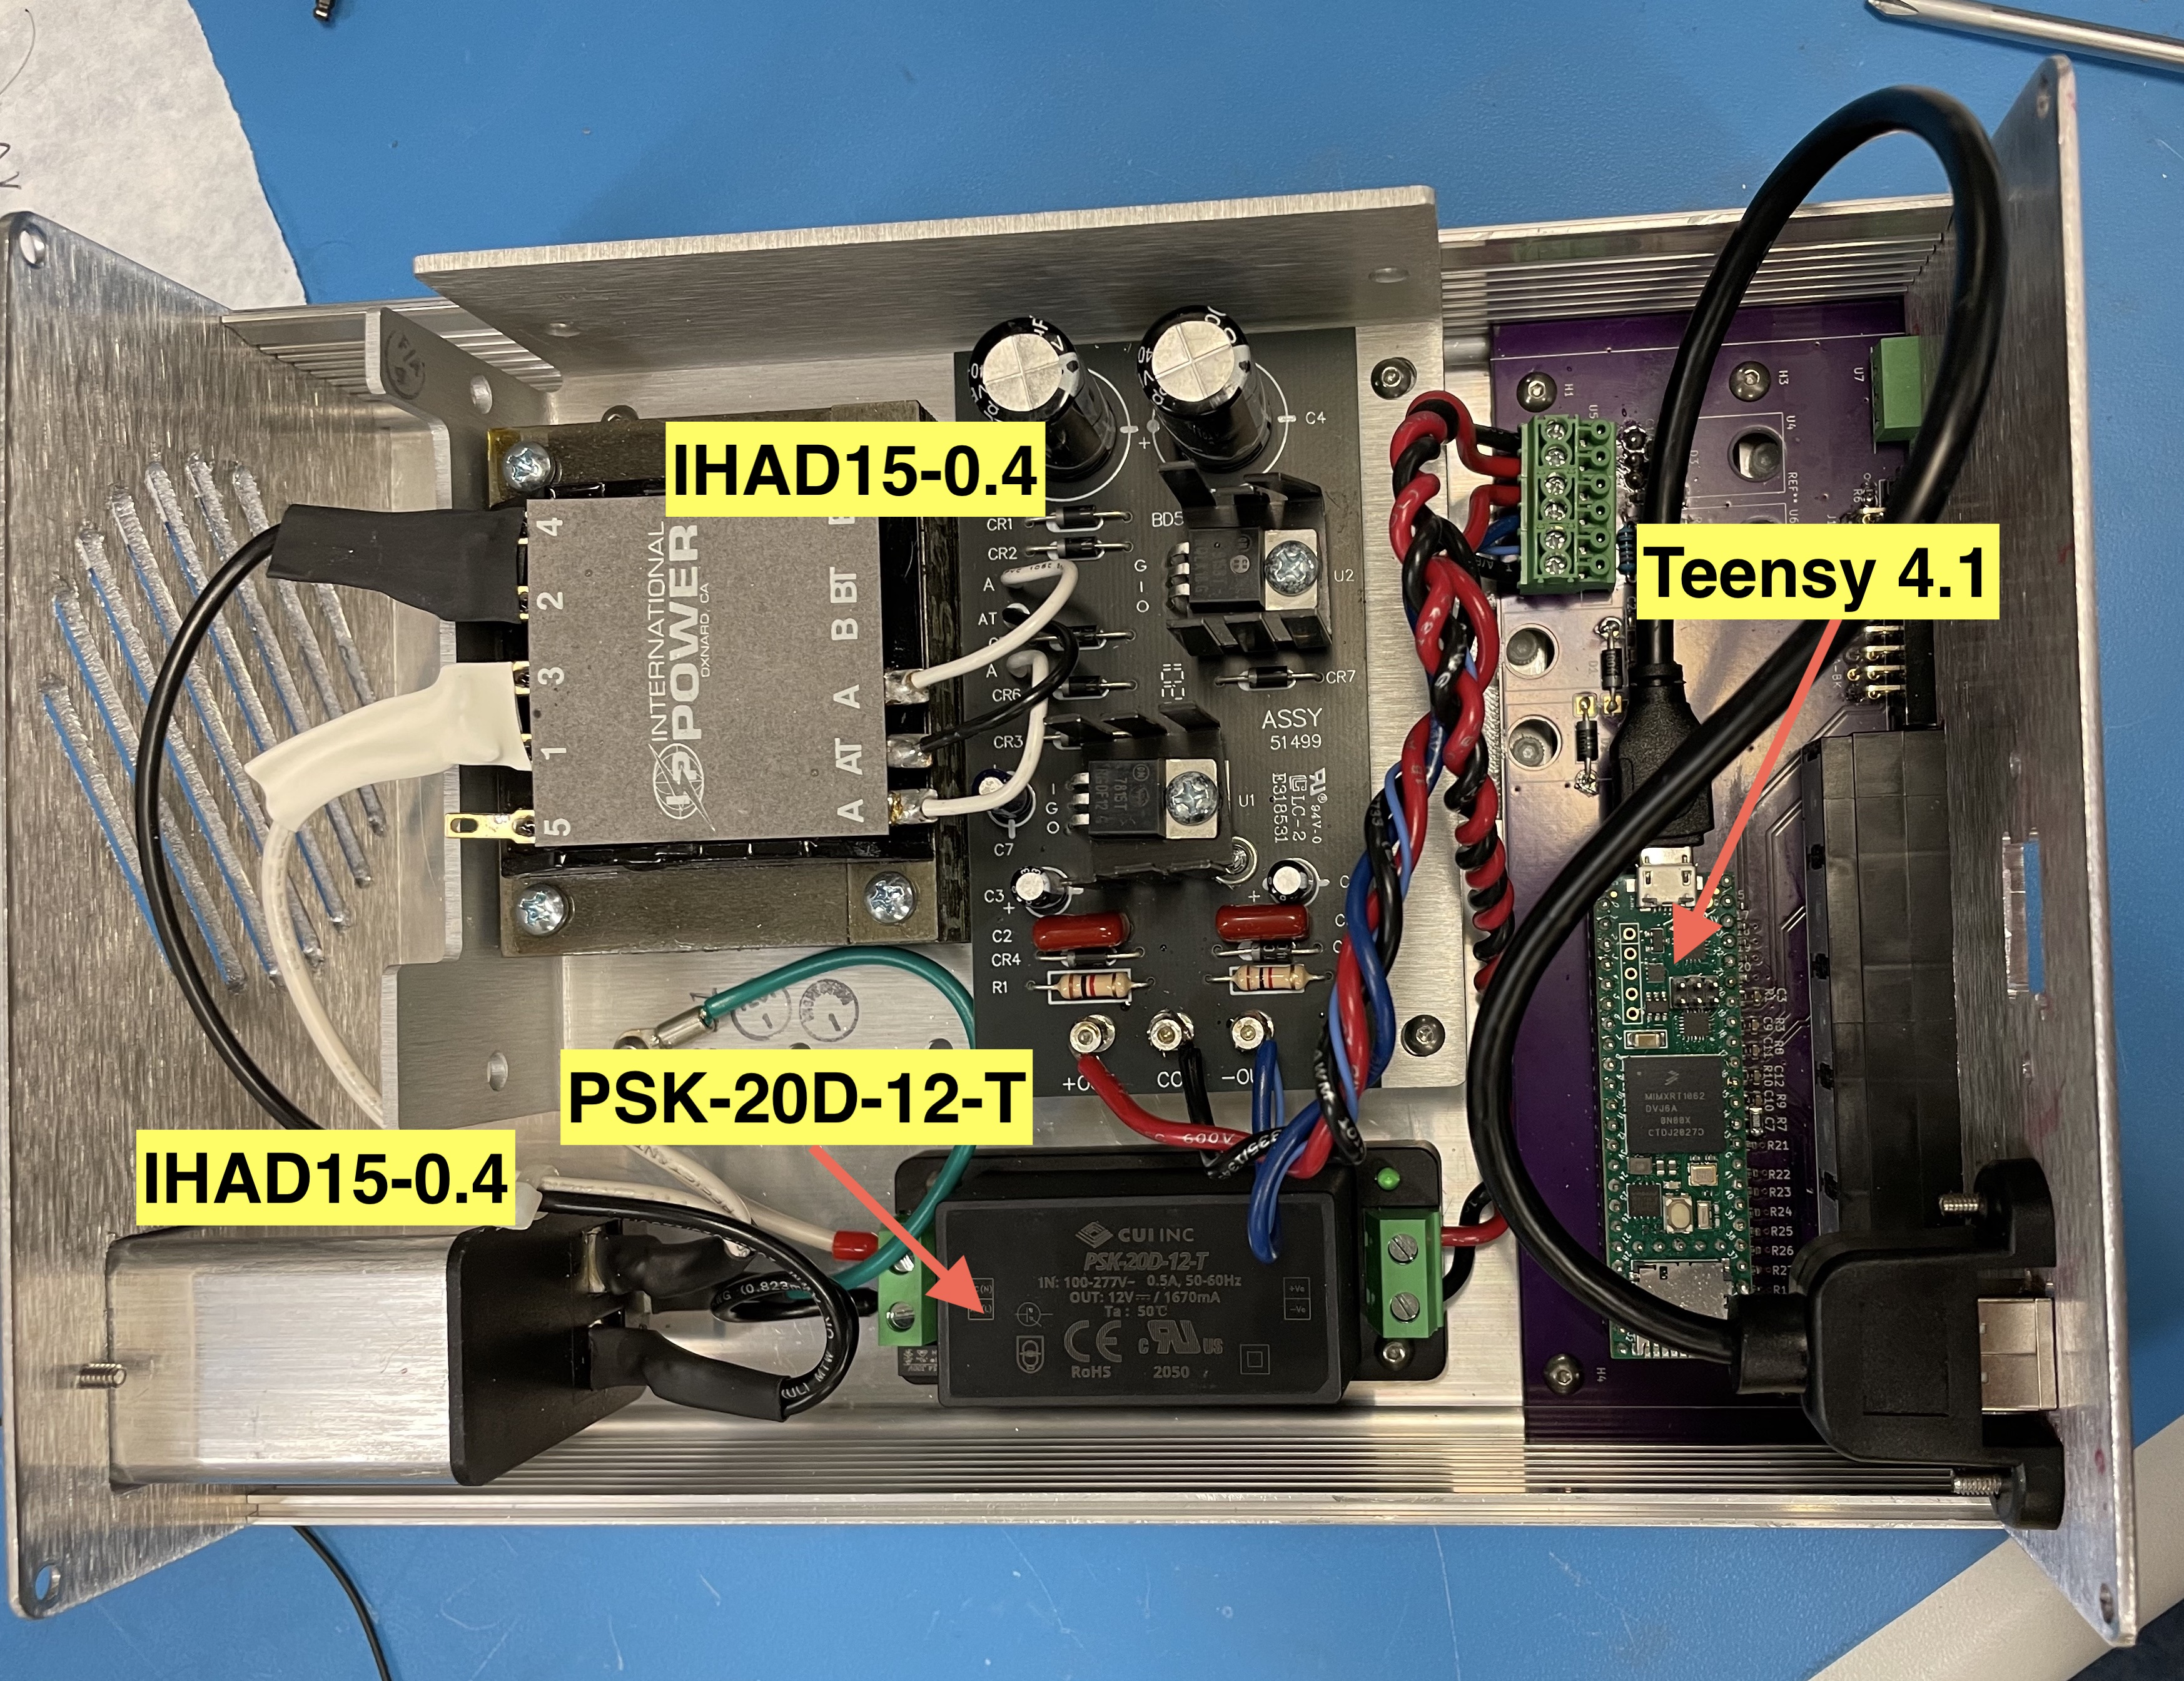
\includegraphics[width=.8\textwidth]{refs_figures/motherboard_box.jpg}
    \caption{The inside of the motherboard box is shown with the power entry module, the two power supplies, and the Teensy labeled with part numbers.}
    \label{motherboard_box}
\end{figure}
The device consists of 3 main components: the optical setup, the motherboard box, and the users computer. The motherboard box, shown in figure \ref{motherboard_box}, contains a Teensy 4.1 microcontroller and two power supplies. The box powers the photodiode detectors and receives 6 voltage signals before communicating them to the user's computer through USB serial. This section will walk through the steps to prepare the device for a measurement. 

\subsection{Optics}
The fiber launch on the polarimeter's optical breadboard is connected to a VOA50-APC variable optical attenuator. This attenuator works for 40nm bands around 1310nm and 1550nm. By turning the screw on the VOA, the input intensity of the light can be adjusted to prevent saturation of the detectors. Each photodiode detecotor will saturate at 130$\mu$W. Therefore, the total input power should be less than $\sim 390\mu$W. 

\subsection{Electronics}
There are two PCB designs used in this device: the Teensy motherboard and the photodiode TIA boards . They were designed in KiCad and the schematics and layouts can be accessed by opening the \verb|.kicab_pro| files.

The 6 photodiode detectors connect to the motherboard box with CAT-5 cables. They need to be connected in order. The connectors on the box are labeled 1 through 6. The detectors should be plugged into the detectors corresponding to the labels in figure \ref{detector_numbers}. 

\begin{figure}[h]
    \centering
    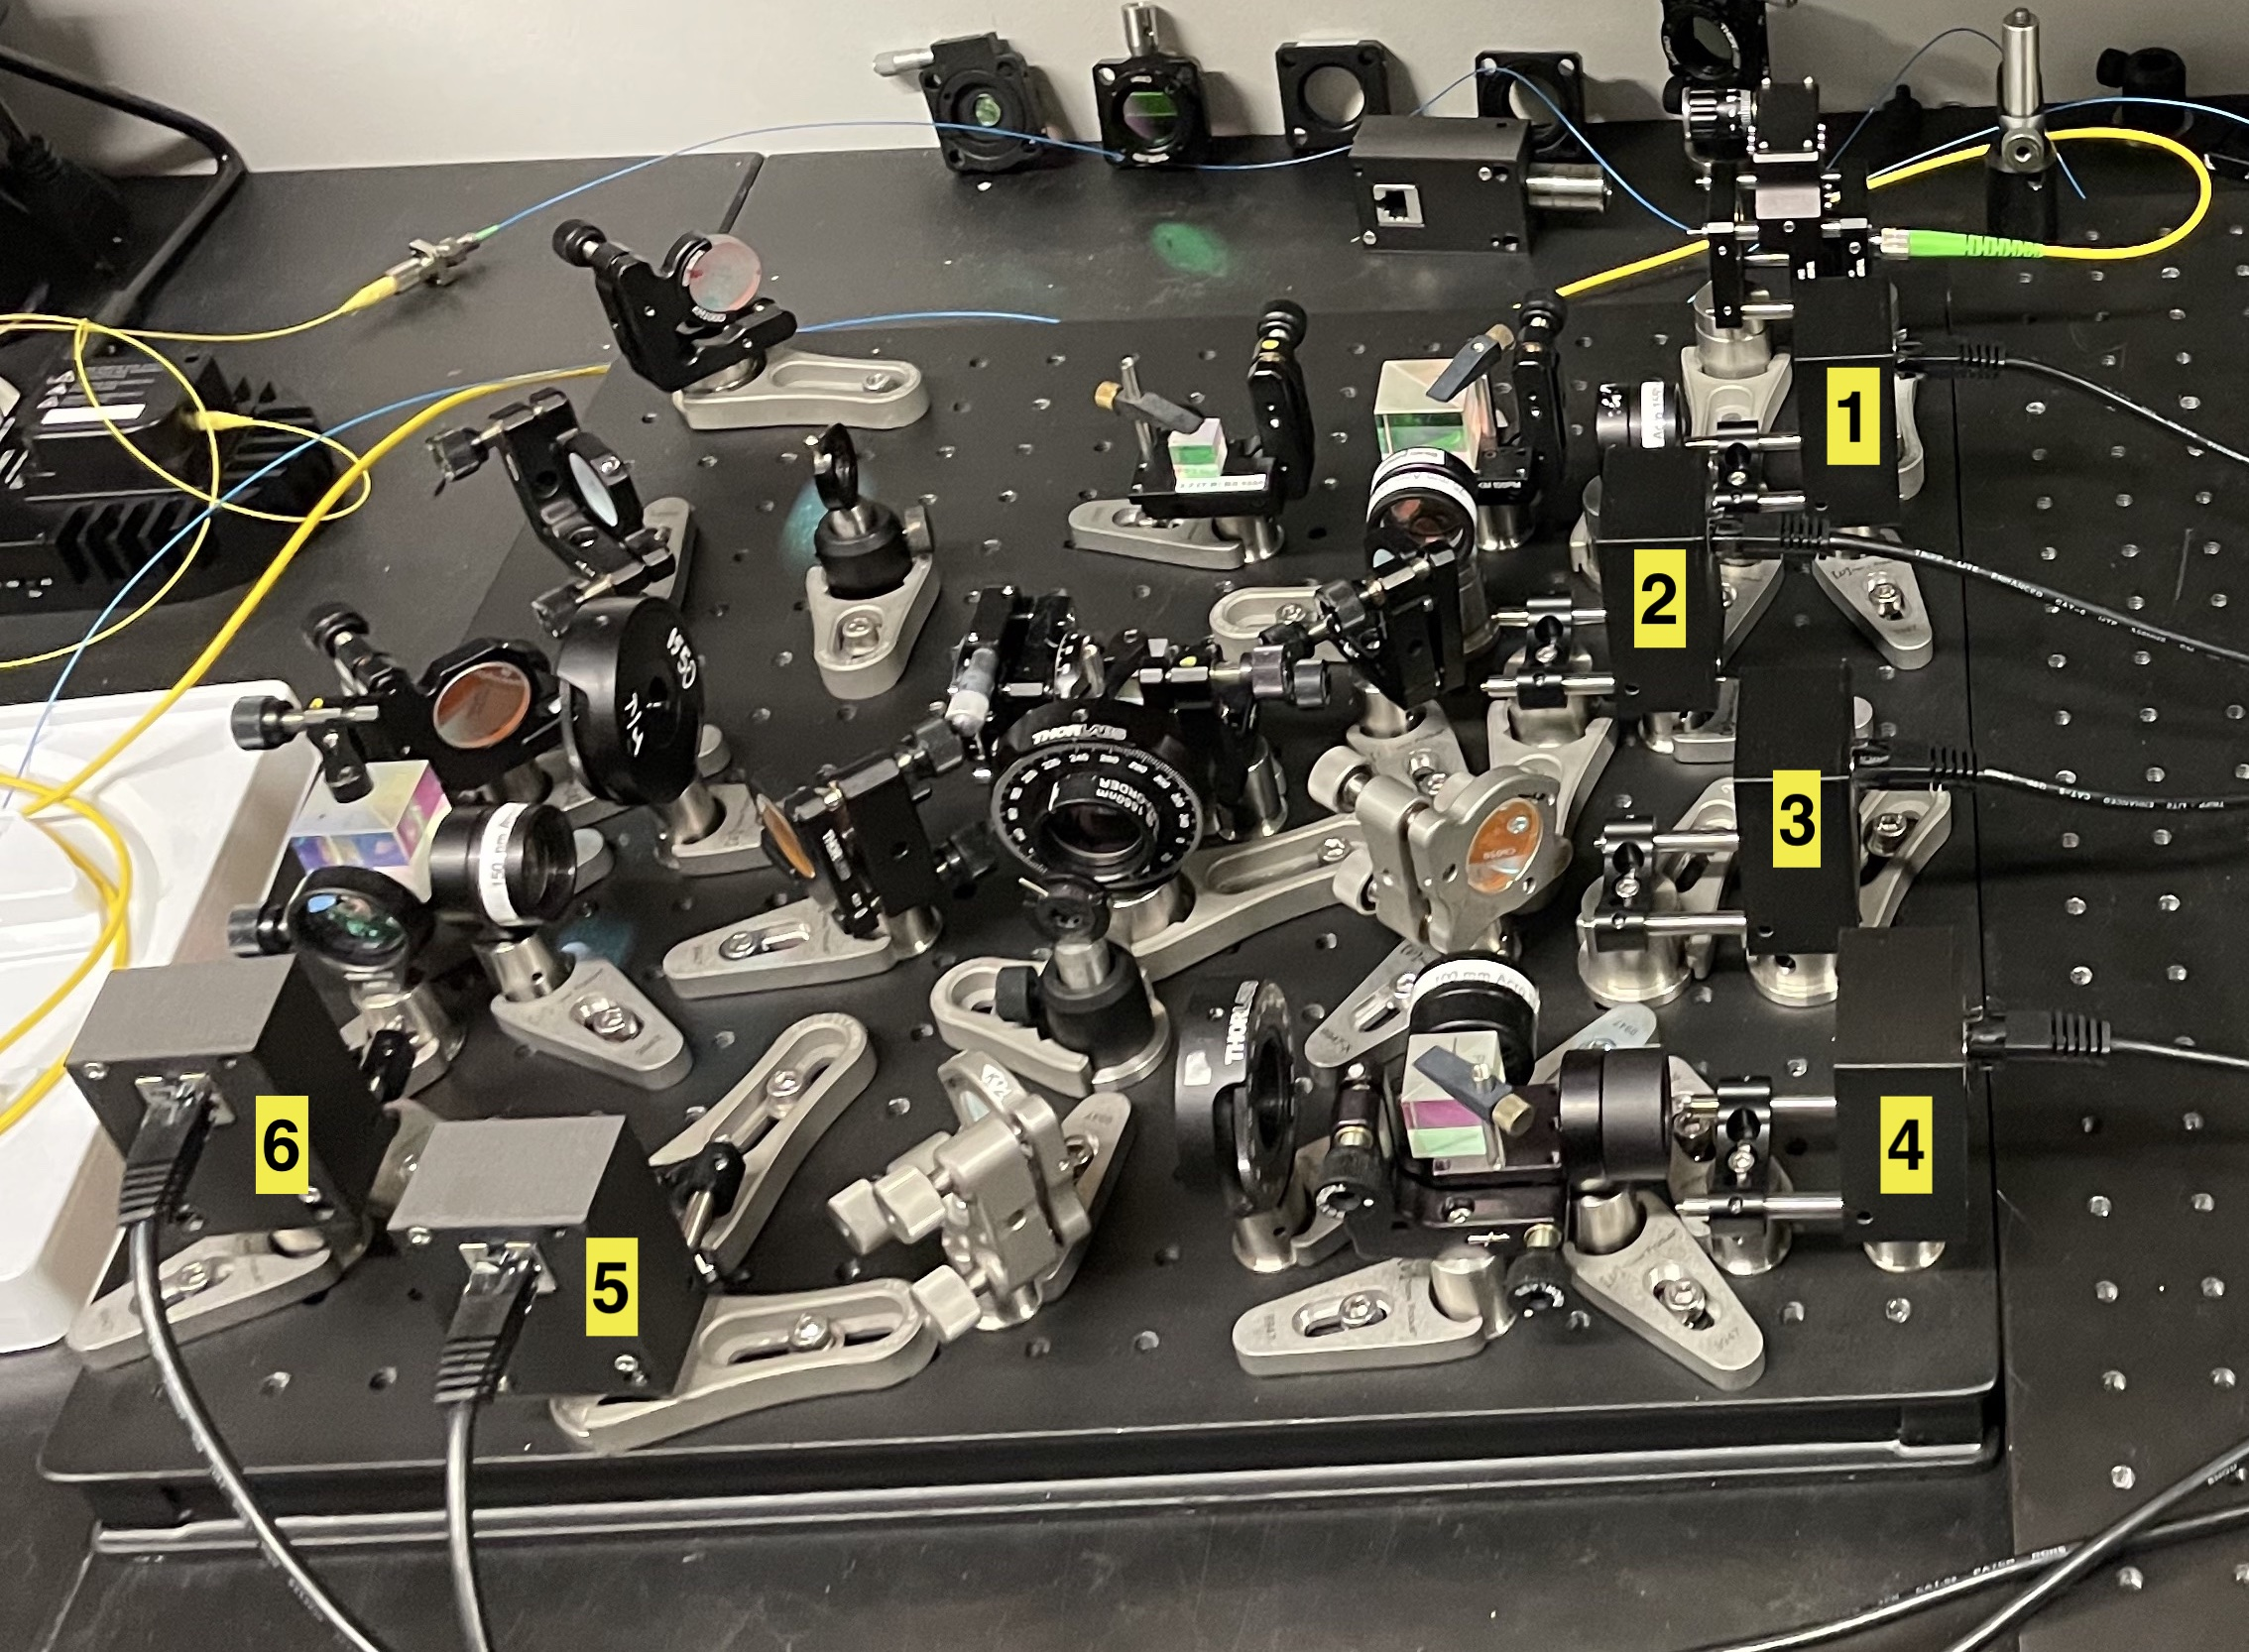
\includegraphics[width = 0.7\textwidth]{refs_figures/DetectorNumbers.jpg}
    \caption{The detectors should be connected to the motherboard box with this numbering.}
    \label{detector_numbers}
\end{figure}

The box needs to plugged into a wall outlet with a power cord and then connected to a computer by a USB cable.

\subsection{Software}
To operate the device, the Teensy 4.1 in the motherboard box and the user's computer need to be running compatible scripts that communicate through serial. The Teensyduino IDE can be used to upload \verb|.ino| scripts to the microcontroller. This can be downloaded from the \href{https://www.pjrc.com/teensy/td_download.html}{PJRC website}. \verb|SerialParallel.py| and \verb|DriftMeasurement.ino| can be used to make polarization measurements for a specified range of time. \verb|SerialParallel.py| takes the file name for the data and a number of measurements for the detector to take. With the current implementation, the number should be a multiple of 50,000. The device's sample rate is $\sim10$kHz so the number of measurements can be used to roughly set the duration of the measurement. The output of the measurement will be a CSV file containing the 6 voltage measurements from sample. This can be converted to polarization measurements with the most up to date calibration matrix. At the writing of this manual, this matrix is the following. 
 \begin{verbatim}
        Binv = np.matrix([
        [ 0.194, 0.241, 0.255, 0.235, 0.283, 0.273],
        [-0.788, 0.871, 0.0227, 0.0310, -0.0961 ,-0.0594],
        [ 0.110 , -0.142, 0.793, -0.819, 0.103, -0.107],
        [ 1.54, -1.694, 0.524, -0.619, -1.56, 1.97]])
 \end{verbatim}
The text above can be directly copied into a python script to produce a numpy matrix of $\textbf{B}^{+}$. This calibration matrix was calculated on 8/5/2022.

\section{Calibration}
The calibration is done in 2 stages. First, a linear polarizer is used to generate a series of known linear polarization states. The input polarization state can be calculated with the angle of the transmission axis of the polarizer from vertical $\theta$ with Equation \ref{input states}.
\begin{equation}
\vec{S}_{linear} =
\begin{bmatrix}
S_0\\
S_1\\
S_2\\
S_3
\end{bmatrix}=
I(\theta)\begin{bmatrix} 
1\\
-cos(2\theta)\\
sin(2\theta)\\
0
\end{bmatrix}
\label{input states}
\end{equation}
The intensity output from the polarizer will in practice be a function of the rotation angle. From equations \ref{Calibration eq} and \ref{input states}, the $i^{th}$ component of $\Vec{V}$ can be expressed as a linear combination of matrix elements $b_{ij}$. 

\begin{equation}
    v_i = I(\theta) \left( b_{i1} - b_{i2}cos(2\theta) + b_{i3}sin(2\theta) \right)
\end{equation}

The original calibration was done with a linear polarizer with a measured extinction ratio of $>1000:1$ and the orientation of the transmission axis known to $\sim\pm0.25\degree$. The linear polarizer was mounted in a motorized rotation mount and rotated continuously through $360\degree$ at a rate of $1\degree$ per second. The polarimeter recorded measurements at 10,000 Hz. The laser used for this generated linearly polarized light so a waveplate was used to produce circular polarization to input to the polarizer to make intensity of as uniform as possible throughout the measurement. The dependence of the intensity on the polarizer angle could not be completely eliminated so a second data set was taken that measured the intensity after the polarizer as it rotated through $360\degree$s, $I(\theta)$. Then  A chi squared fit to the measured $v_{i}$ was used to determine the $b_{ij}$ matrix elements.

 The second stage of the calibration requires input states with some known ellipticity. For this, a procedure presented in \cite{Azzam89} was used to account for the error in these input states. First, a linear polarizer and a quarter waveplate were aligned with the transmission axis of the former rotated by $45\degree$ from fast axis of the latter. In practice, this produces a nearly circular state. Represented on the Poincare sphere, this state is slightly displaced from one of the poles in figure \ref{Poincare Sphere}. Then, by rotating both the linear polarizer and the quarter waveplate by $90\degree$, the input state is rotated by 180 degrees around the north-south axis of the Poincare sphere. If the initial state was close to circular, then the average of these two states is nearly aligned to the pole of the Poincare sphere and hence a perfect circular state. The input polarization states are linearly related to the voltage states so the voltage states can be averaged to calculate the detectors response to a perfect circular state. To carry out this procedure, $\Vec{V}_1$ and $I_1$, the voltage state and output intensity from the first input state, were measured. After rotating by $90\degree$, $\Vec{V}_2$ and $I_2$ were measured. Then equation \ref{V_circ} was used to calculate the detectors response to normalized circular input state. 
 \begin{equation}
     \Vec{V}_{circ} = \frac{1}{2} \left( \dfrac{\Vec{V_1}}{I_1} + \dfrac{\Vec{V_2}}{I_2} \right)
     \label{V_circ}
 \end{equation}
Then, the last column of the matrix can be calculated.
\begin{equation}
    B_4 = \pm V_{circ} - B_1
    \label{last_col}
\end{equation}
Here, $B_i$ represents that $i^{th}$ column of the instrument matrix and the sign is positive if the circular state generated was right-handed. With the instrument matrix determined, the calibration matrix can be calculate with equation \ref{MP_inverse}. 

For the calibration performed on 5/8/2022, the results are compared to the theoretical values in Figure \ref{calibration Data}. Good agreement can be seen between the theoretical curves and the measured curves for the normalized Stokes parameters. 
\begin{figure}[!h]
\begin{center}
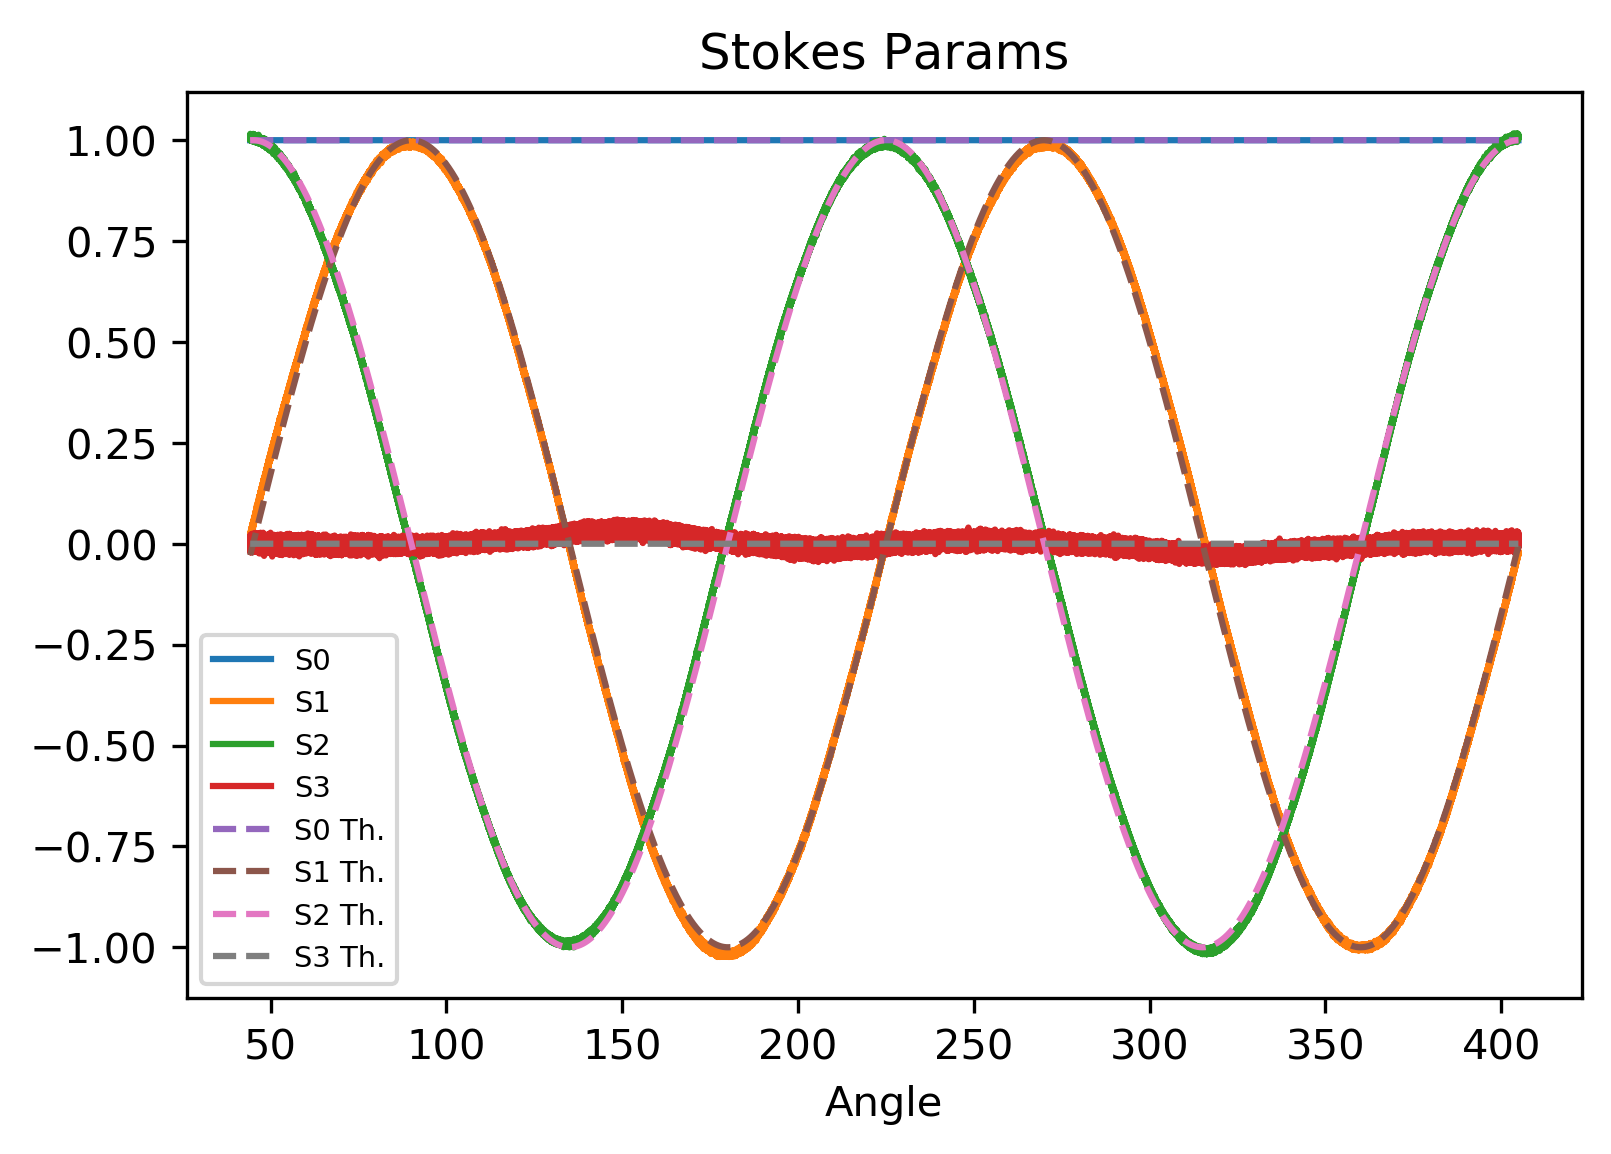
\includegraphics[width=0.7\textwidth]{refs_figures/Calibration Data.png}
\end{center}
\caption{The normalized Stokes parameters are graphed. The measured parameters are solid lines and the theoretical parameters are dotted lines.}
\label{calibration Data}
\end{figure}

\verb|1550 Calibration Analysis Pt 2.ipynb| was used to analyze the data taken during the calibration procedure and calculate the $\textbf{B}^{+}$. \verb|780CalibrationAnalysis.ipynb| was used for 780 nm version of the polarimeter so the calculations can also be referenced. 

\section{Notes}
\subsection{Calibration and wavelength dependence}
The waveplates in used are a mix of single and multi order waveplates. Therefore, the device is expected to have wavelength dependent performance and should be calibrated on the wavelength needed for a measurement. This may be improved by replacing the waveplates with achromatic waveplates. 
\subsection{Teensyduino IDE}
The Teensyduino IDE is a valuable tool for working with the polarimeter. It allows for simple serial communication between the user's computer and the Teensy. The Serial Monitor and Serial Plotter functions allowed for the data sent from the Teensy to be visualized and plotted. \verb|Photodiode_Mode.ino| sends the voltages from each photodiode to the user's computer in the so that the Serial Plotter will automatically plot these values as a funtion of time. This has many use cases, including tuning the input power so that none of the photodiodes saturate.



\section{Acknowledgements}
This device was built during the summer of 2022 in the Rubidium Rydberg lab with advisors Dr. Steven Rolston and Dr. Trey Porto. Credit and thanks are owed to Patrick Banner for his involvement and mentroship and Dr. Alessandro Restelli for his invaluable electronics help.





\printbibliography
\end{document}
